\documentclass{article}
\usepackage[utf8]{inputenc}

\title{Laboratorio03_INTELIGENCIA_NEGOCIOS}
\author{edwartbalcon}
\date{Septiembre 2021}

\usepackage[utf8]{inputenc}
\usepackage[spanish]{babel}
\usepackage{natbib}
\usepackage{graphicx}

\begin{document}

\title{Caratula}

\begin{titlepage}
\begin{center}
\begin{Large}
\textbf{UNIVERSIDAD PRIVADA DE TACNA} \\
\end{Large}
\vspace*{-0.025in}
\begin{figure}[htb]
\begin{center}

\includegraphics[width=6cm]{./images/logo_UPT}
\end{center}
\end{figure}
\vspace*{-0.025in}
\begin{Large}
\textbf{FACULTAD DE INGENIERIA} \\
\end{Large}
\vspace*{0.05in}
\begin{Large}
\textbf{Escuela Profesional de Ingeniería de Sistema} \\
\end{Large}


\vspace*{0.4in}

\vspace*{0.1in}
\begin{Large}
\textbf{Informe de laboratorio 05: Elaboración de reportes Operacionales} \\
\end{Large}

\vspace*{0.3in}
\begin{Large}
\textbf{Curso: Inteligencia de negocios} \\
\end{Large}

\vspace*{0.3in}
\begin{Large}
\textbf{DOCENTE: Ing. Patrick Cuadros Quiroga} \\
\end{Large}

\vspace*{0.2in}
\vspace*{0.1in}
\begin{large}

\begin{Large}
\textbf{Alumno: Balcon Coahila, Edwart Juan\hfill	(2013046516) } \\
\end{Large}

\vspace*{0.15in}
\begin{Large}
\textbf{Tacna – Perú} \\
\end{Large}

\vspace*{0.05in}
\begin{Large}
\textbf{2021 } \\
\end{Large}

\end{large}
\end{center}

\end{titlepage}


\newpage
    \section{}
    \subsection{Parte I: Crear la fuente de datos}
    \begin{enumerate}[\tab 1.]
        \item Abrir datastudio.google.com e iniciar sesión con su cuenta de Google
        \begin{center}
            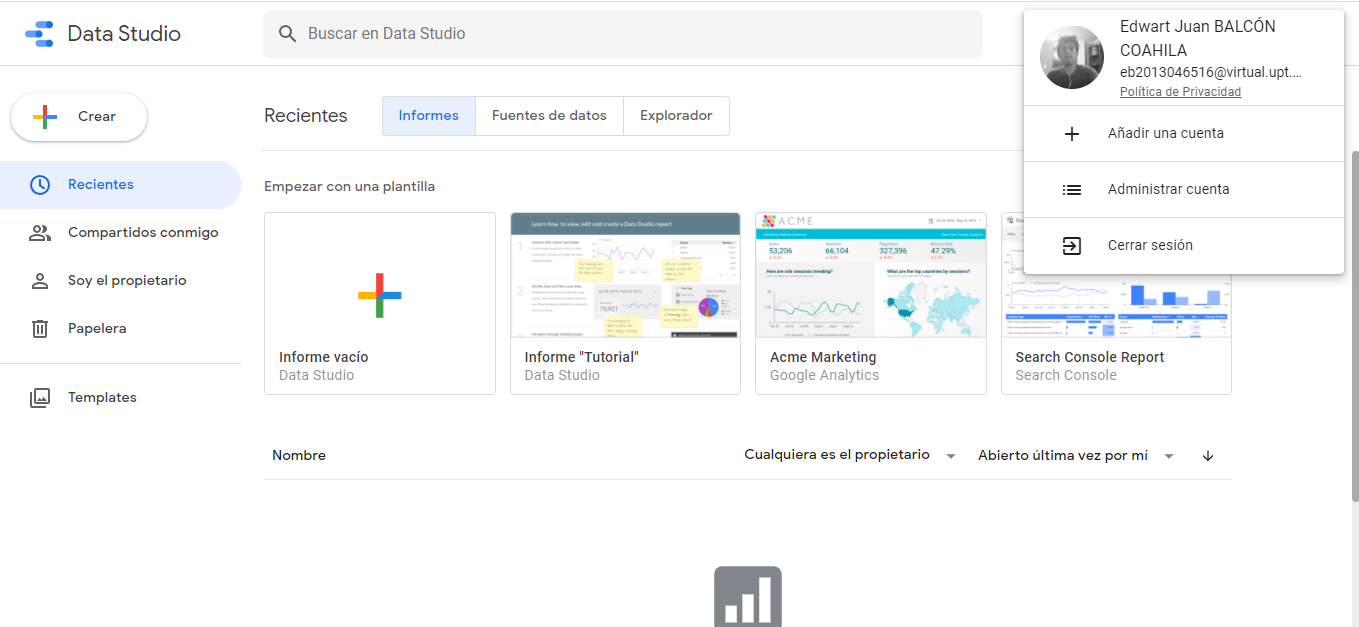
\includegraphics[width=13cm]{./images/1.png}
        \end{center}
        
            \item Abrir Google Drive y crear una hoja de calculo de Google Sheet en blanco
            \begin{center}
                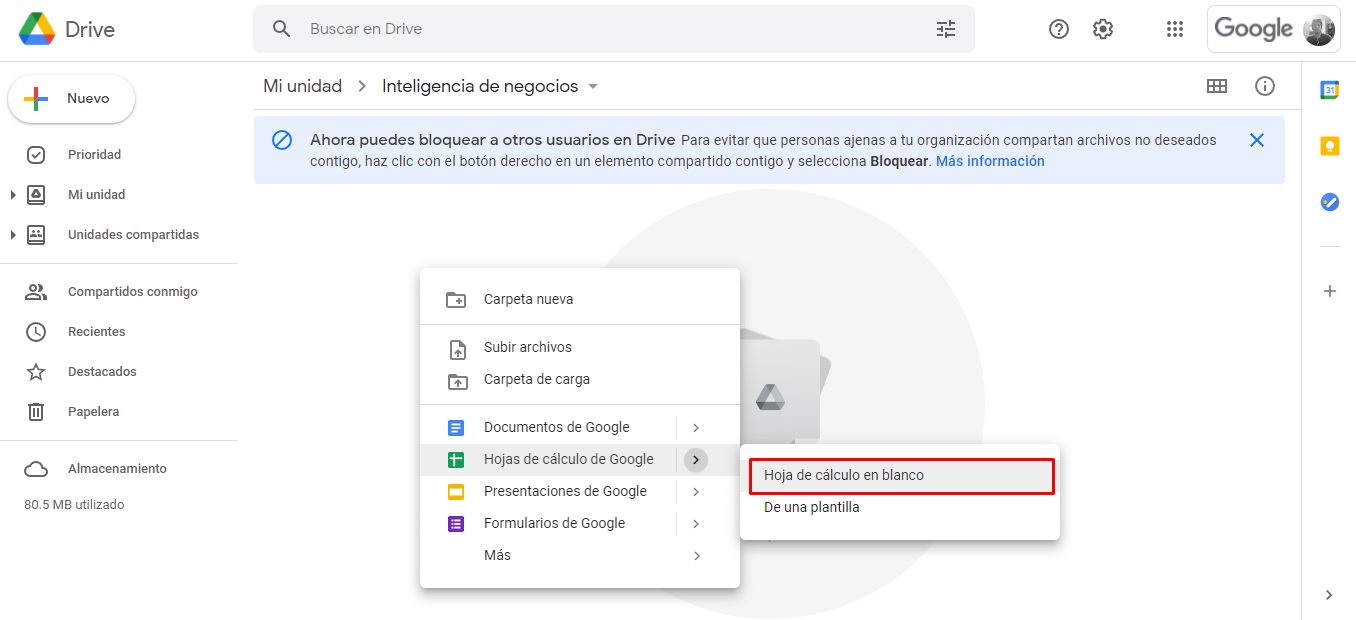
\includegraphics[width=13cm]{./images/2.png}
            \end{center}
            \newpage
            \item Renombrar la hoja “Covid Data”
            \begin{center}
                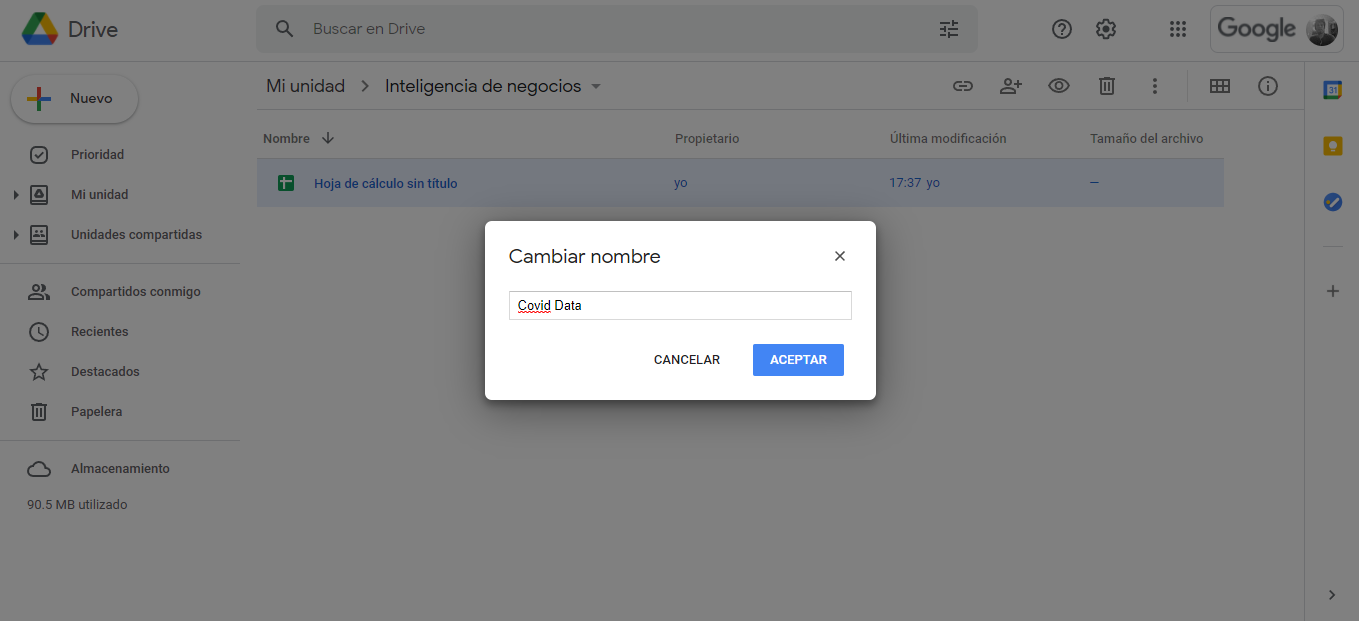
\includegraphics[width=13cm]{./images/3.png}
            \end{center}
            \item  En la primera celda, escribir la formula
=IMPORTHTML("https://www.worldometers.info/coronavirus/", "table",1)
            \begin{center}
                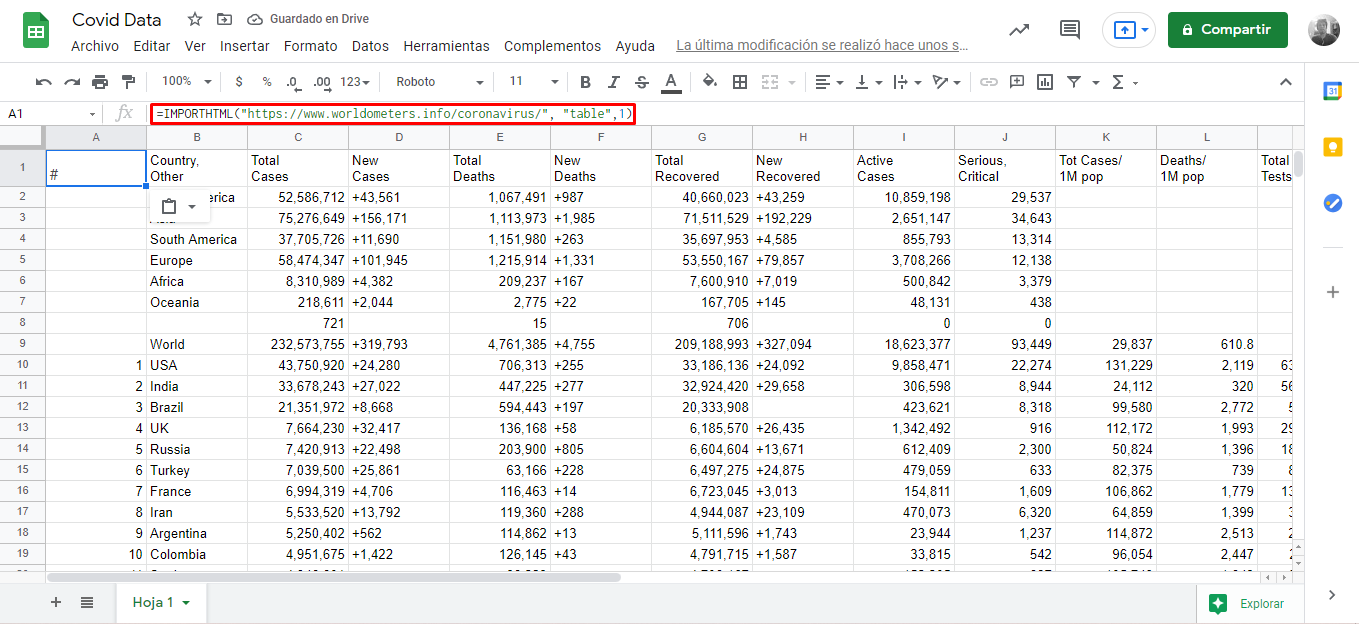
\includegraphics[width=13cm]{./images/4.png}
            \end{center}
        \newpage
    \end{enumerate}
    
    \subsection{Parte II: Crear el Origen de Datos}
    \begin{enumerate}[\tab 1.]
        \item En Data Studio, haga click en el botón Crear y selecciones Informes
        \begin{center}
            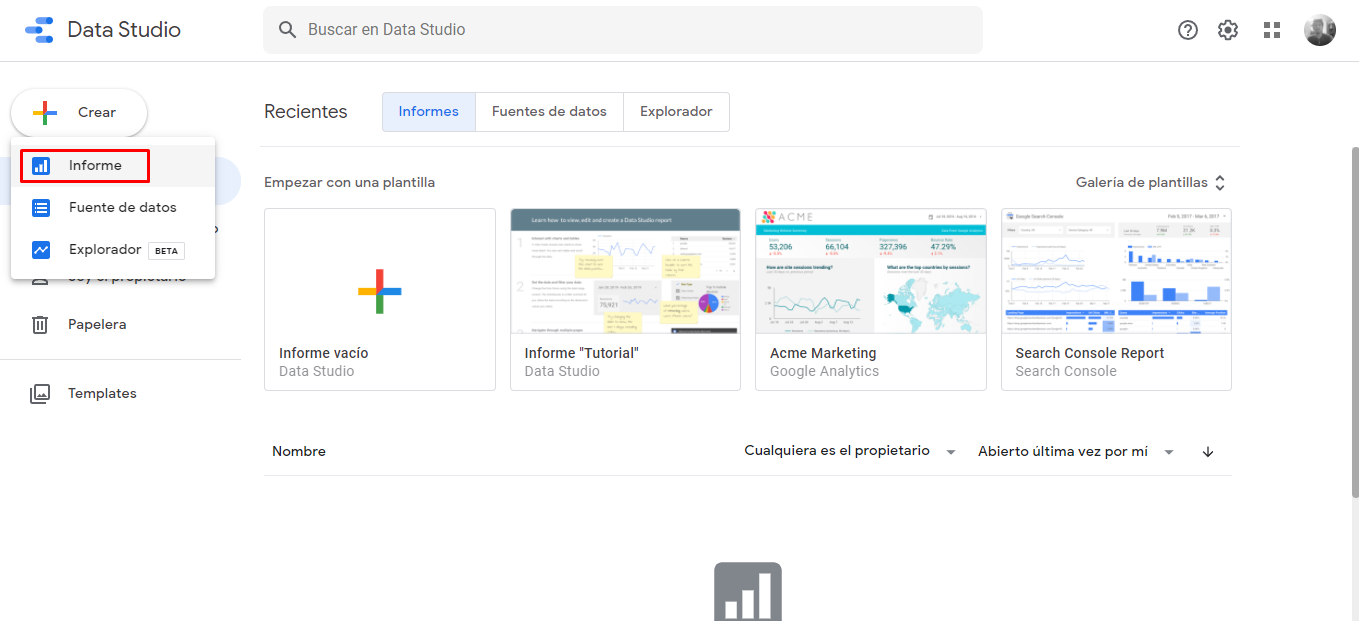
\includegraphics[width=13cm]{./images/5.png}
        \end{center}
        
        \item Completar las opciones de primera vez
        \begin{center}
            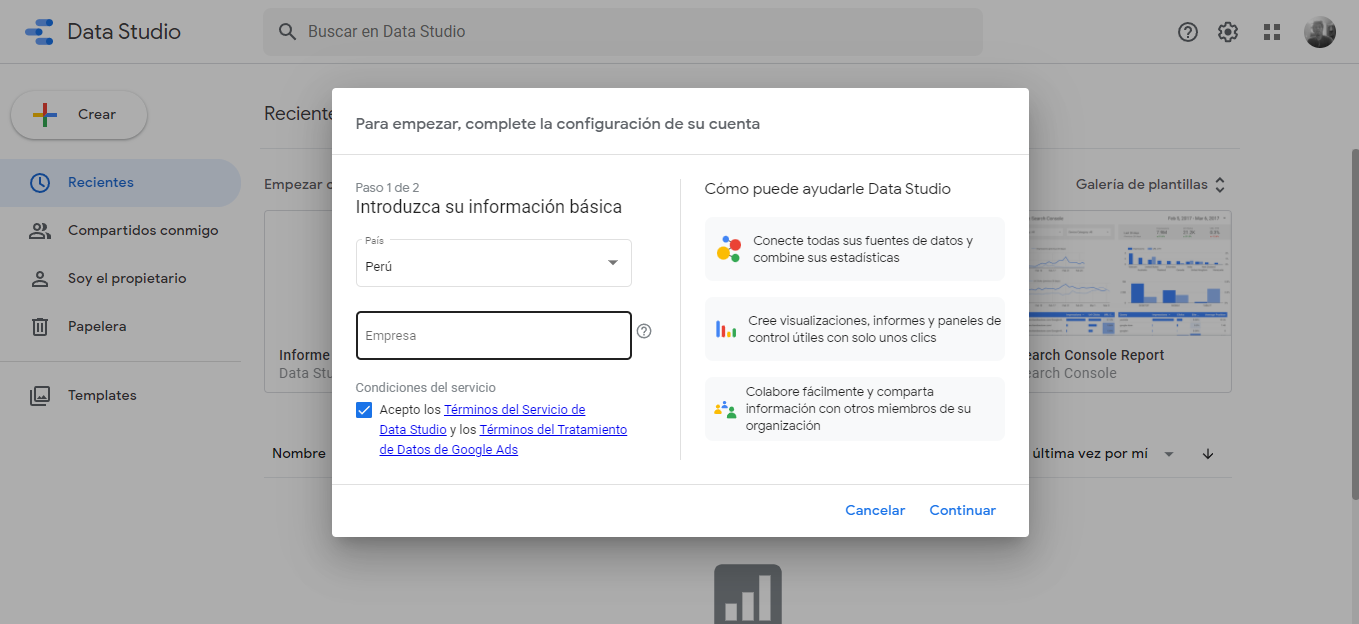
\includegraphics[width=13cm]{./images/6.png}
        \end{center}
        \newpage
        \item Seleccionar el conector Google Sheet y añadir la hoja “Covid Data”
        \begin{center}
            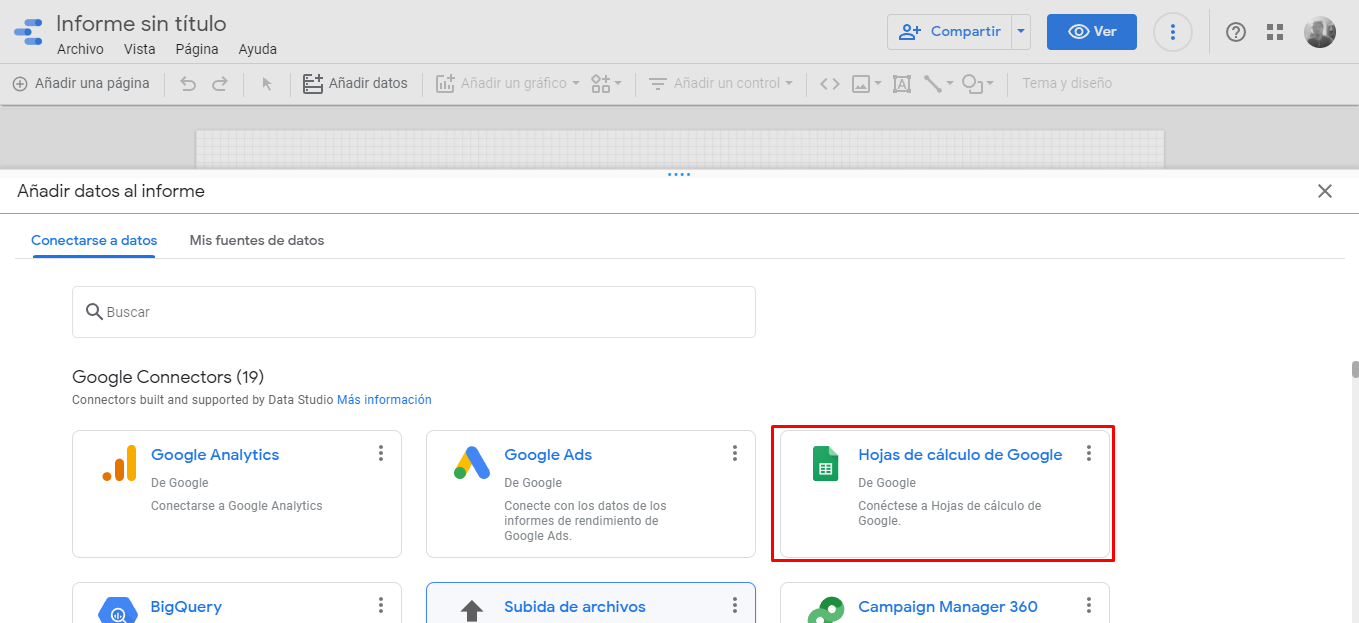
\includegraphics[width=13cm]{./images/7.png}
        \end{center}
        \begin{center}
            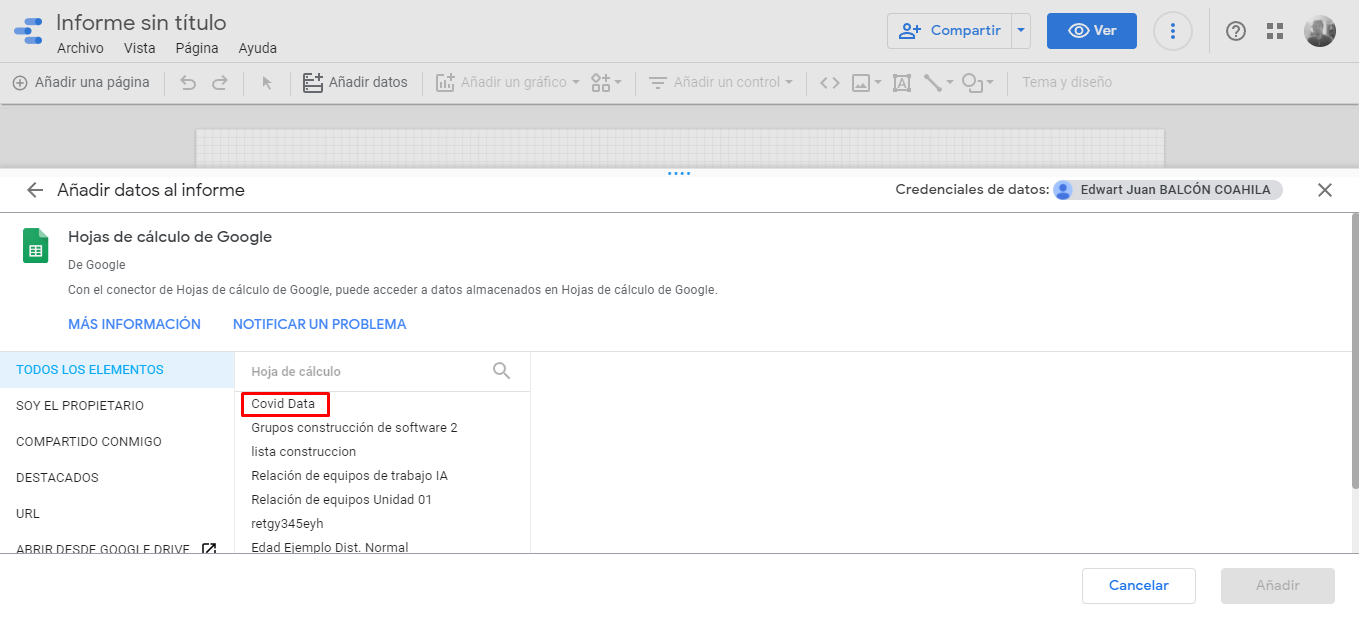
\includegraphics[width=13cm]{./images/8.png}
        \end{center}
       \newpage
        \item Ocultar las filas no deseadas en la hoja y desmarcar la opción "Incluir celdas ocultas y filtradas” y luego hacer click en Añadir reporte o Conectar
        \begin{center}
            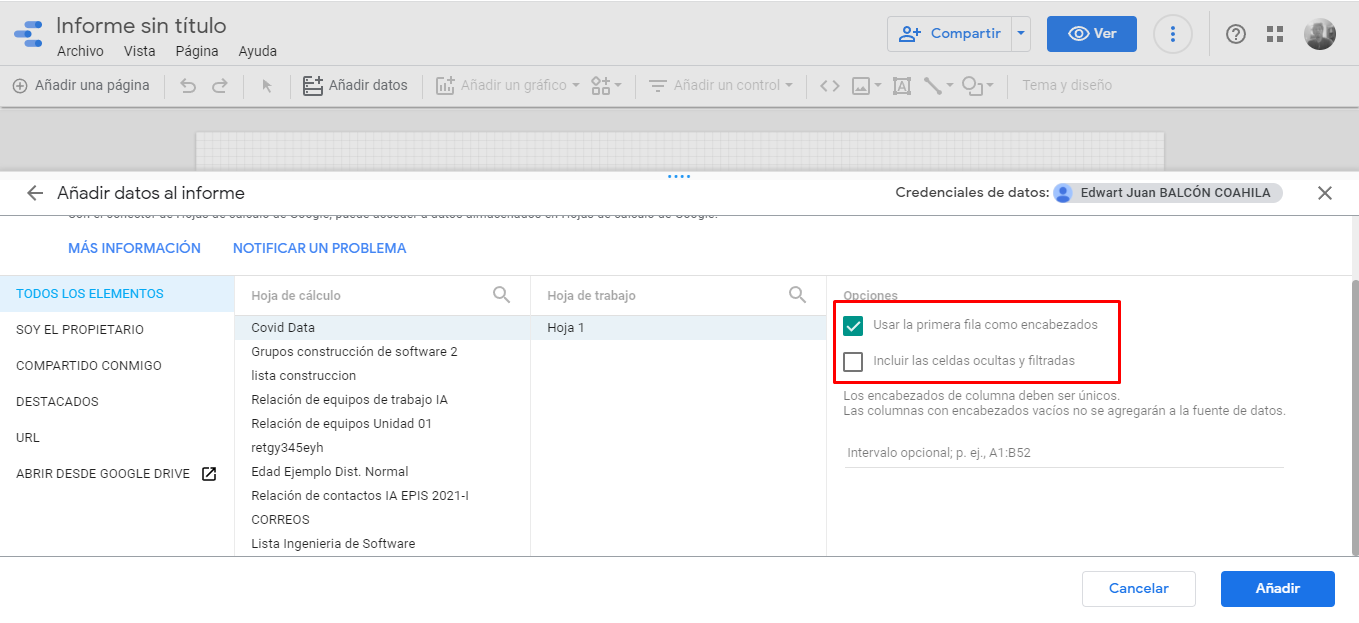
\includegraphics[width=13cm]{./images/9.png}
        \end{center}
        
    \end{enumerate}
    \newpage
    \subsection{Parte III: Añadir campos al origen de datos}
    \begin{enumerate}[\tab 1.]
        \item En el menú Recurso, abrir “Gestión de las fuentes de datos añadidas” y click en Editar
        \begin{center}
            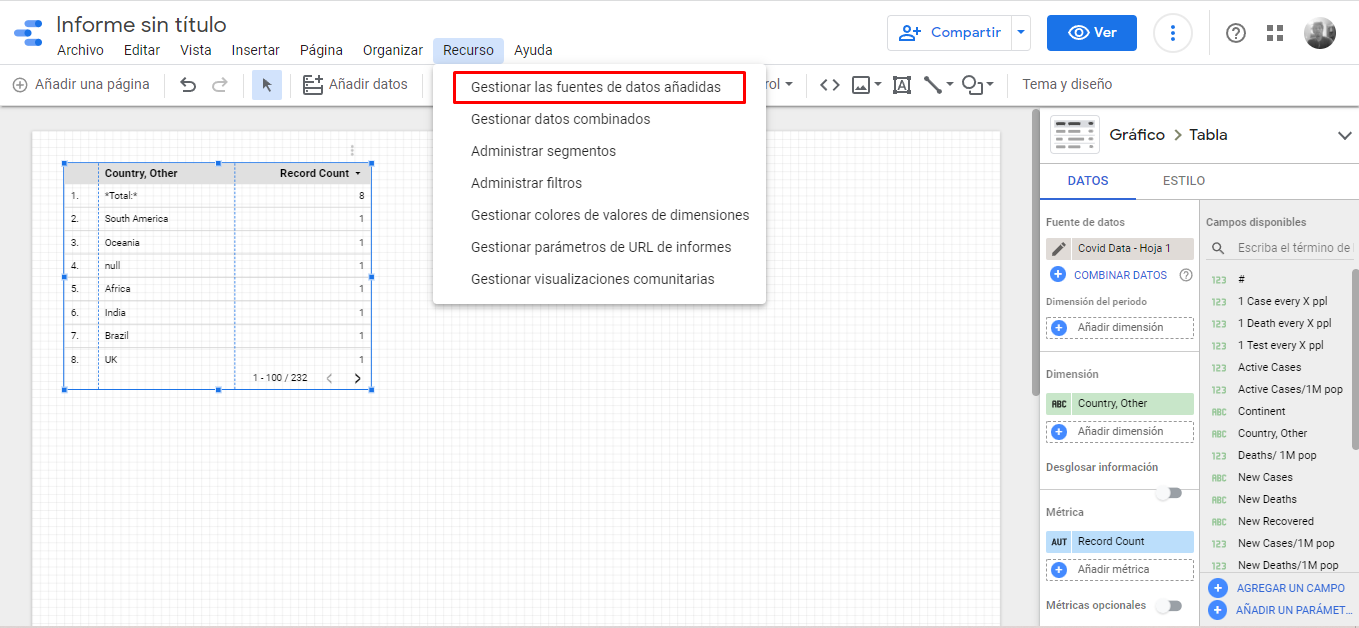
\includegraphics[width=13cm]{./images/10.png}
        \end{center}
        \begin{center}
            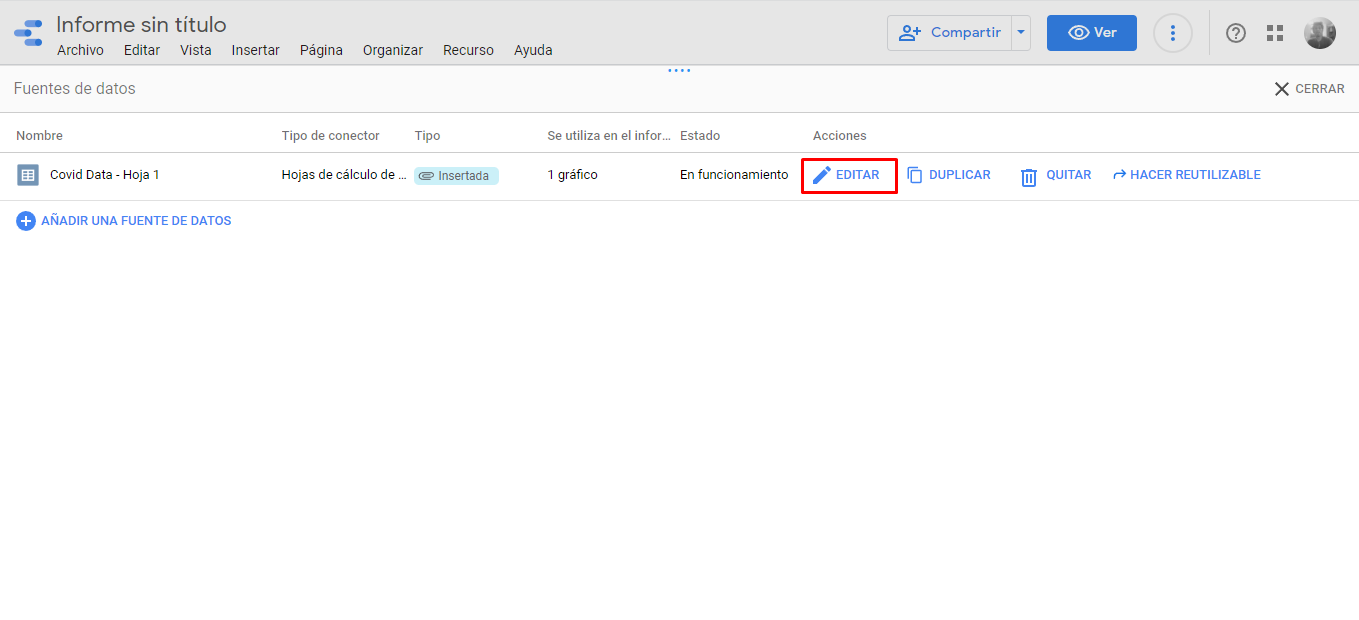
\includegraphics[width=13cm]{./images/11.png}
        \end{center}
        \newpage
        \item Verificar los datos y sus tipos de datos “Omega”.
        \begin{center}
            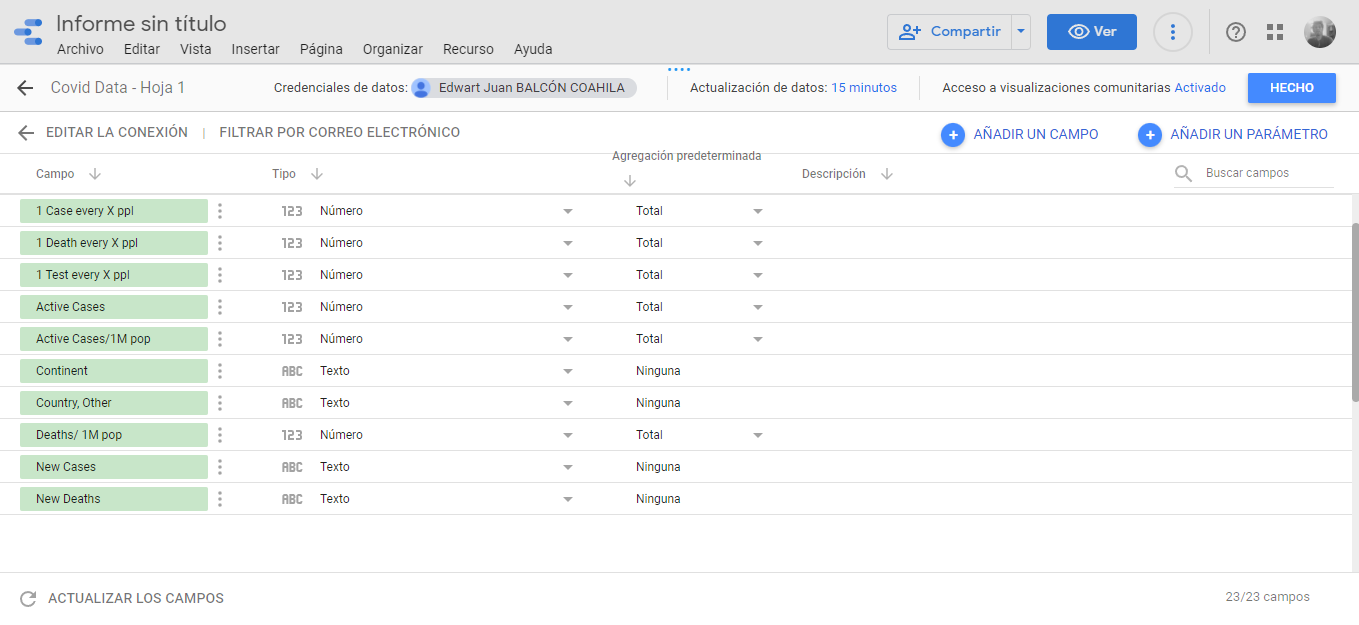
\includegraphics[width=13cm]{./images/12.png}
        \end{center}
        \item Deshabilitar el campo Conteo o cantidad de registros o filas
        \begin{center}
            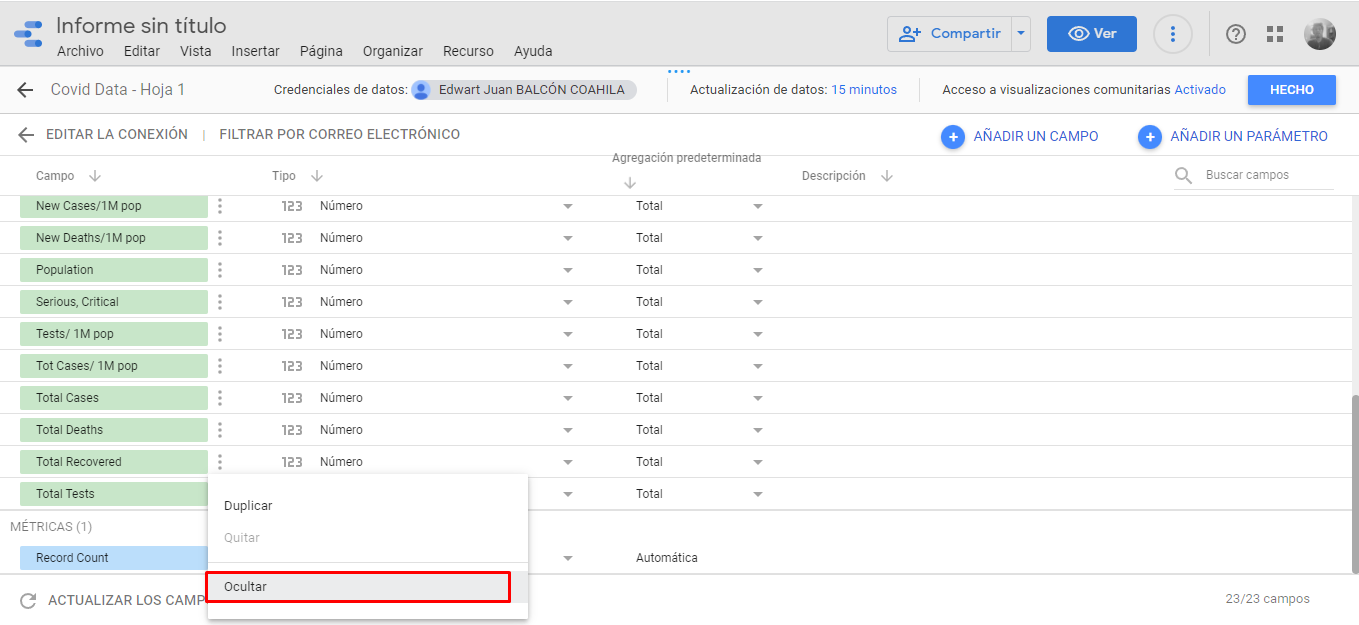
\includegraphics[width=13cm]{./images/13.png}
        \end{center}
        \newpage
        \item Crear dos nuevos Campos: Casos mundiales
        \begin{center}
            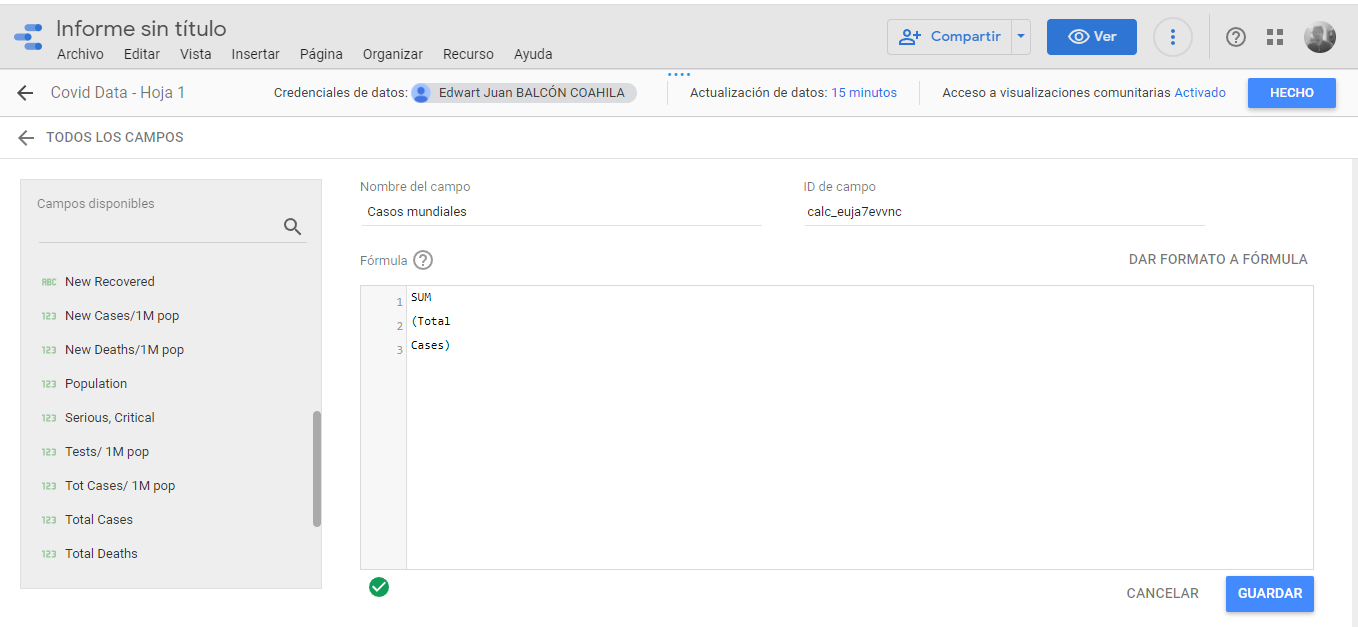
\includegraphics[width=13cm]{./images/14.png}
        \end{center}
        \newpage
        \item Crear dos nuevos Campos: Tasa de mortalidad
        \begin{center}
            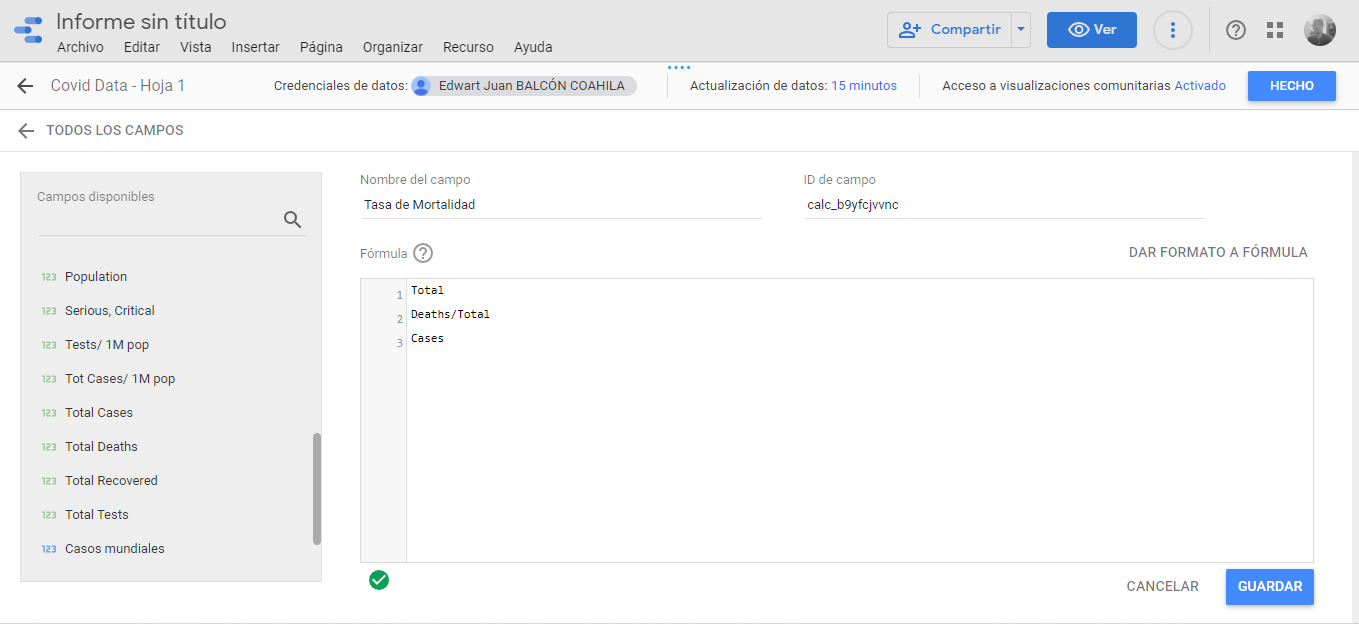
\includegraphics[width=13cm]{./images/15.png}
        \end{center}
       
    \end{enumerate}
    
    \subsection{Parte IV: Crear Diferentes Dashboards}
        \begin{center}
            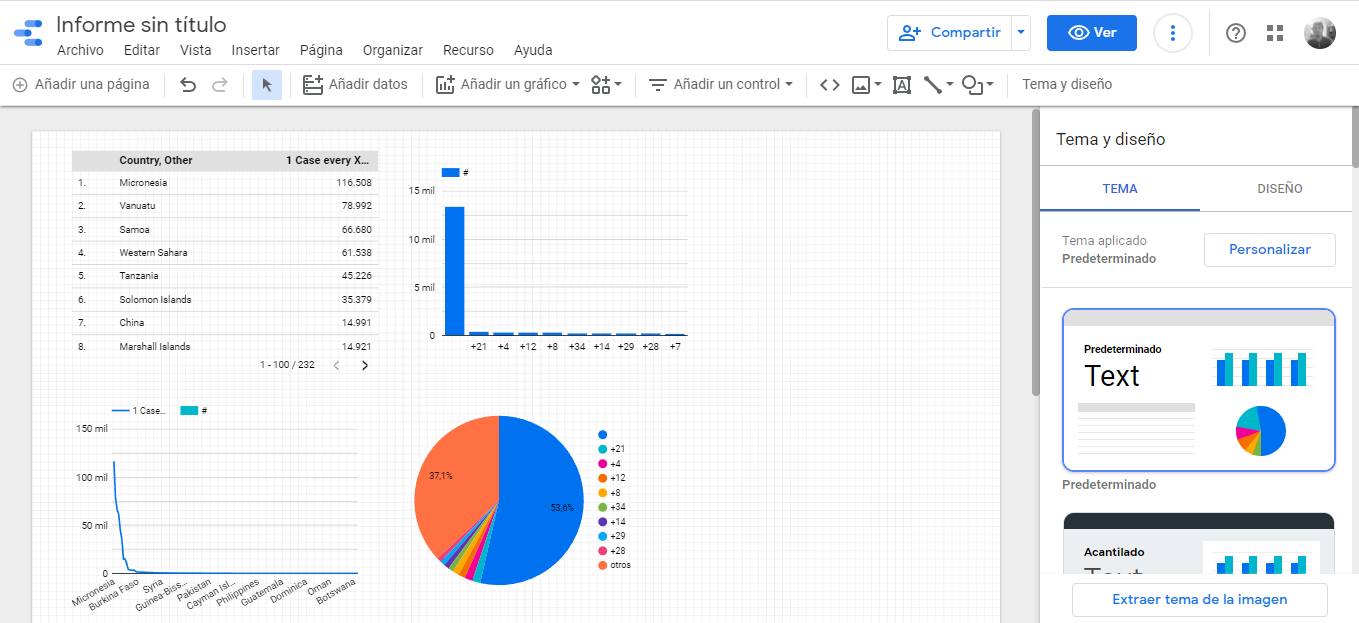
\includegraphics[width=13cm]{./images/16.png}
        \end{center}


	
\end{document}